\subsection{Handling Halo cells}
\label{subsec:handling-halo-cells}

Proper handling of tile boundaries is crucial to ensure the accuracy of our Sobel computation. As depicted in Figure~\ref{fig:tile-boundary}, neglecting to process tile boundaries appropriately results in assigning a value of 0.0 to pixels along the shared tile edges. 

To address this issue, halo cells are incorporated into the computation. During the scatter phase, halo cells are sent along with the data tiles. These halo cells are then utilized during the Sobel processing phase to ensure seamless computation across tile boundaries. It is important to note that halo cells are not transmitted back during the gathering phase.

\begin{figure}[h!]
    \centering
    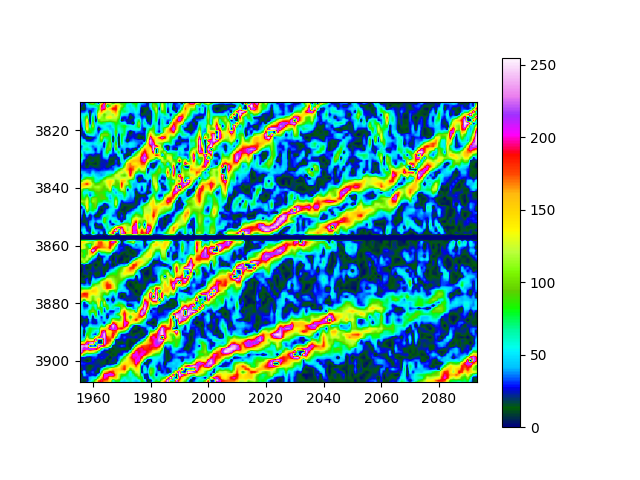
\includegraphics[width=\linewidth]{images/tile-boundary.png}
    \caption{Illustration of tile boundaries without appropriate halo cell processing.}
    \label{fig:tile-boundary}
\end{figure}